\documentclass[11pt,a4paper]{article}

\usepackage{amsmath}
\usepackage{graphicx}
\usepackage{epstopdf}

\title{AMTH250 \\ Assignment 8}

\author{Mark Villar}

\begin{document}

\maketitle

\subsubsection*{Question 1} 
\begin{enumerate}

	\item[(a)] $$I_1=\int^{\infty}_0 \frac{x^3}{e^x-1} \ dx = 6.4939$$
	\begin{center}
		\includegraphics[width=0.55\textwidth]{f1.eps}
	\end{center}

	\item[(b)] $$I_2=\int^1_{-1} \ln(1+x)\ln(1-x) \ dx = -1.1016$$
	\begin{center}
		\includegraphics[width=0.55\textwidth]{f2.eps}
	\end{center}
	
	\item[(c)] $$I_3=\int^{\pi}_0 \tan(\sin x)-\sin(\tan x) \ dx = 2.6643$$
	\begin{center}
		\includegraphics[width=0.6\textwidth]{f3.eps}
	\end{center}
	These results are reliable since $I_1, I_2$ and $I_3$ were successfully evaluated with an absolute error tolerance of $10^{-13}, 10^{-13}$ and $10^{-12}$ respectively.
	
	\begin{verbatim}
		f1=@(x) x.^3./(e.^x-1);
		[intf1,ierr,nf,eerr]=quad(f1,0,Inf,[1e-13 0])
		intf1 =  6.4939
		ierr1 = 0
		nf1 =  345
		eerr1 = 7.8500e-014
	
		f2=@(x) log(1+x).*log(1-x);
		[intf2,ierr2,nf2,eerr2]=quad(f2,-1,1,[1e-13 0])
		intf2 = -1.1016
		ierr2 = 0
		nf2 =  735
		eerr2 = 6.2172e-015

		f3=@(x) tan(sin(x))-sin(tan(x));
		[intf3,ierr3,nf3,eerr3]=quad(f3,0,pi,[1e-12 0])
		intf3 =  2.6643
		ierr3 = 0
		nf3 =  735
		eerr3 = 5.9641e-013
	\end{verbatim}
\end{enumerate}

\pagebreak

\subsubsection*{Question 2}
$$C(x)=\int^x_0 \cos\left(\frac{\pi t^2}{2}\right) \ dt$$
\begin{center}
	\includegraphics[width=0.55\textwidth]{fresc.eps}
\end{center}
$$S(x)=\int^x_0 \sin\left(\frac{\pi t^2}{2}\right) \ dt$$
\begin{center}
	\includegraphics[width=0.55\textwidth]{fress.eps}
\end{center}
$$\text{Cornu or Euler spiral}$$
\begin{center}
	\includegraphics[width=0.55\textwidth]{cornu.eps}
\end{center}
\subsubsection*{Question 3}
\begin{enumerate}
	\item[(a)] We first identify the range of random numbers for each dimension.
	$$x \in [0,1], \ y \in [0,2], \ z \in [0,4]$$
	Then we enclose the ellipsoid in a $4 \times 4$ cube. We select $n=100000$ points uniformly distributed within the cube and use the distance formula 
	$$d=\sqrt{\left(\frac{x}{a}\right)^2+\left(\frac{y}{b}\right)^2+\left(\frac{z}{c}\right)^2}$$ 
	to check whether the point is contained within the ellipsoid. If $d \le 1$, then the given point is inside the ellipsoid. We then estimate the volume of the ellipsoid by the formula
	$$V_e \approx V_c \times \frac{k}{n}=\frac{64k}{n}$$
	where $V_c$ is the volume of the cube, $k$ is the number of points in the ellipsoid and $n$ is the number of points in the cube. Thus, by Monte Carlo approximation 
	$$V_e \approx 33.567$$
	This is consistent with the exact result
	$$V_e=\frac{4}{3}\pi abc = \frac{32}{3}\pi = 33.510$$
	where $a=1, b=2, c=4$.
	
	\item[(b)] Since $\Omega$ is contained within the square $[0,1] \times [0,1]$, we generate $x$ and $y$ as uniform $[0,1]$ random numbers. We then generate $n$ random numbers and use those lying in $\Omega$ to form the sum of the function. Equating the volume of $\Omega$ and the average value of $f$ in $\Omega$, our Monte Carlo integration is given by
	$$I=V_{\Omega} \times \frac{1}{n} \sum^n_{i=1} \sum^n_{j=1} e^{-\sqrt{x^2_i+y^2_j}} \approx 0.83028$$
	where $V_{\Omega}=\dfrac{\pi}{2}$. This is consistent with the exact result obtained from Wolfram.
	$$\int^1_{-1} \int^{\sqrt{1-y^2}}_0 e^{-\sqrt{x^2+y^2}} \ dx \ dy = 0.830138$$
	
\end{enumerate}

\pagebreak

\subsubsection*{Question 4} 
\begin{enumerate}
	\item[(a)] With initial conditions $t_0=0$ and $y(0)=1$, we apply Euler's method under various step sizes, $h=\dfrac{1}{2^k}$ for $1\le k \le 16$, to solve our initial value problem. The numerical solution is displayed in the graph below.
	\begin{center}
		\includegraphics[width=0.7\textwidth]{euler.eps}
	\end{center}
	We also show the error curve below. We can see that the errors are insignificant enough, of the order of $10^{-6}$, for the computed and exact solutions to be barely distinguishable on a graph. Note that the shape of the curve here is trivial.
	\begin{center}
		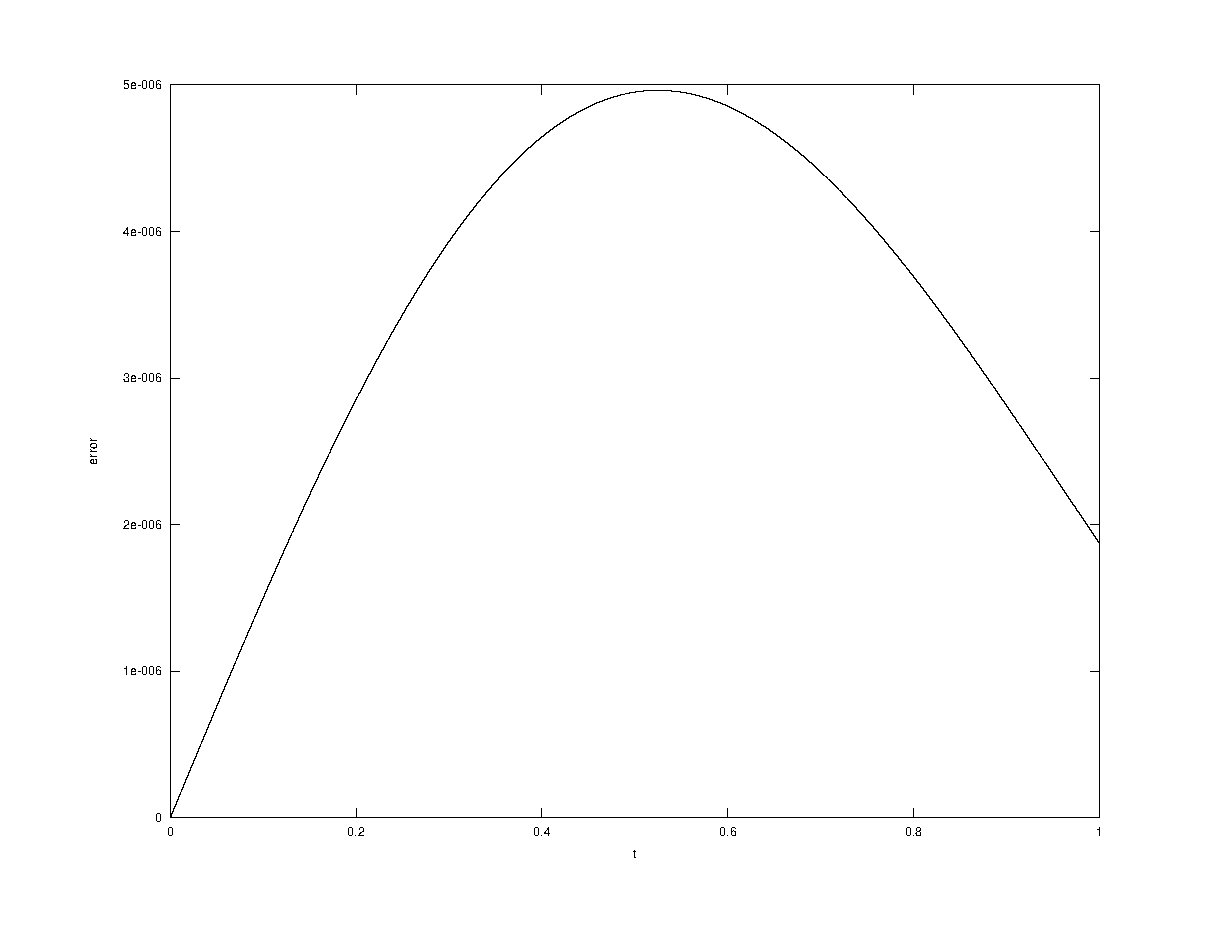
\includegraphics[width=0.7\textwidth]{error.eps}
	\end{center}
	At $t=1$, the exact value of $y(t)$ is $e^{-1} = 0.367879441171442$. We compare this with the computed values from the various step sizes in the table below.
	
	\begin{center}
		\begin{tabular}{|c|c|c|}
		\hline
		$k$ &$y(1)$ &Error \\
		\hline
		1 &0.50000 &0.13212 \\
		2 &0.41016 &0.04228 \\
		3 &0.38571 &0.01784 \\
		4 &0.37613 &0.00825 \\
		5 &0.37185 &0.00398 \\
		6 &0.36983 &0.00195 \\
		7 &0.36885 &0.00097 \\
		8 &0.36836 &0.00048 \\
		9 &0.36812 &0.00024 \\
		10 &0.36800 &0.00012 \\
		11 &0.36794 &0.00006 \\
		12 &0.36791 &0.00003 \\
		13 &0.36789 &0.00001 \\
		14 &0.36789 &0.00001 \\
		15 &0.36788 &0.00000  \\
		16 &0.36788 &0.00000  \\
		\hline
		\end{tabular}
	\end{center}
	
	In fact, at $k=16$, the error is only $1.871 \times 10^{-6}$, which is consistent with our earlier findings. 
	\begin{center}
		\includegraphics[width=0.9\textwidth]{err1.eps}
	\end{center}
	The error curve as a function of $h$ shows that the accuracy of our results improves as we decrease the step size. In other words, the bigger the step size, the larger the error.
	
	\item[(b)] This problem is unstable for $h=1$. We also know by experiment that Euler's method gives `accidental' stable solutions for some larger step sizes, with $y$ decaying to 0 after just a few steps. This is true for $h=1/2$ and $1/4$, converging after only 4 and 10 steps respectively. For this reason we ignore results for $k<2$. Nonetheless, the various step sizes $h=2^{-k}$ for integers $k \ge 3$ all give stable solutions. Thus in general, $h=x^{-k}$ where $x$ is an \emph{exponent of} 2, provide stable results. In other words, 
	$$h=\frac{1}{2^k}, \frac{1}{4^k}, \frac{1}{8^k}, \frac{1}{16^k}, \ldots$$
	are all valid ranges of step-sizes for which $y \rightarrow 0$ as $t \rightarrow \infty$. By trial-and-error we found that for all other $h$, the solution diverges and thus gave unstable result.
	
\end{enumerate}


\pagebreak 

\subsubsection*{Question 5}
\begin{enumerate}
	\item[(a)] $\textbf{lsode}$ solution to the Lorenz system of differential equations
	\begin{center}
		\includegraphics[width=0.65\textwidth]{y1.eps}
	\end{center}
	\begin{center}
		\includegraphics[width=0.65\textwidth]{y2.eps}
	\end{center}
	\begin{center}
		\includegraphics[width=0.65\textwidth]{y3.eps}
	\end{center}
	\pagebreak
	
	\item[(b)] Phase-plane plots 
	\begin{center}
		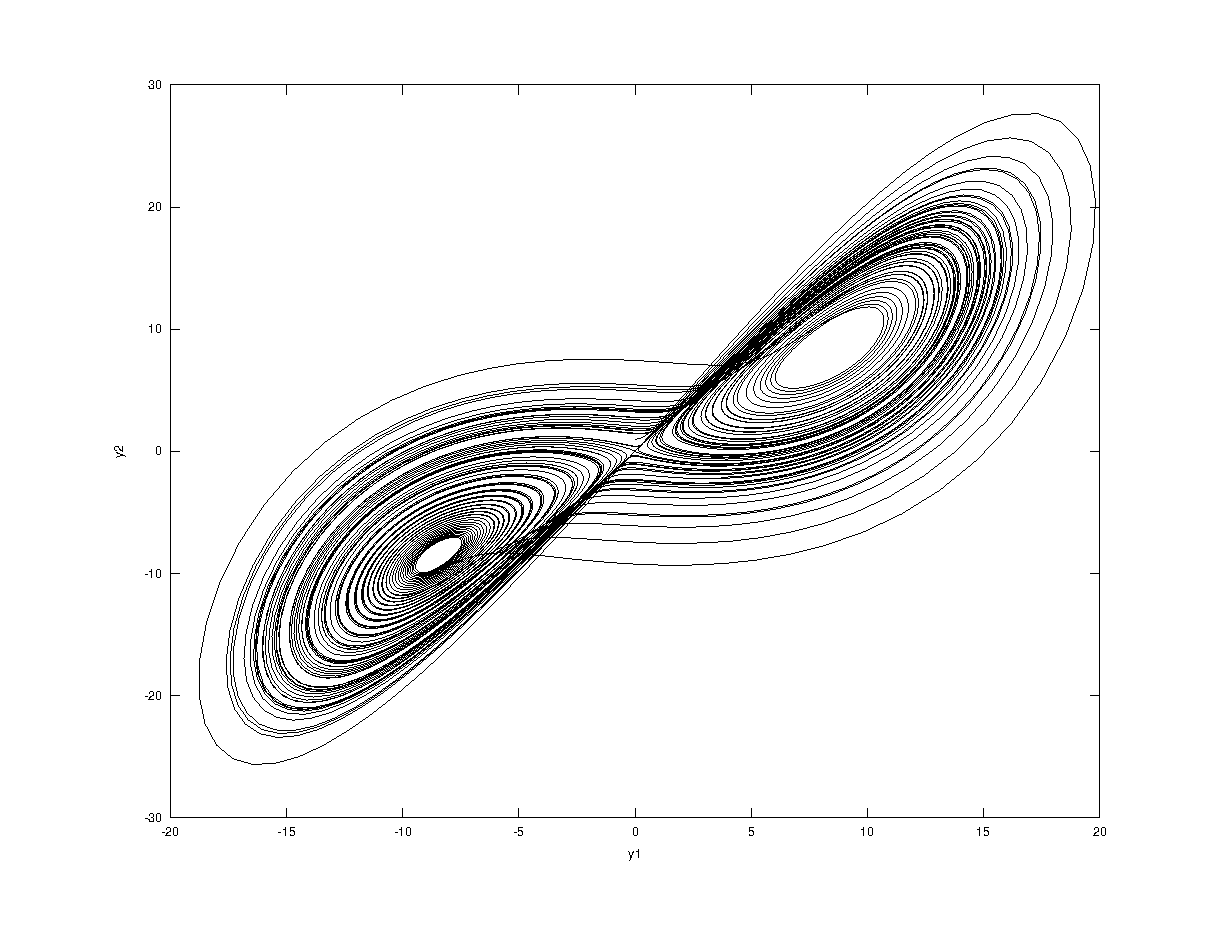
\includegraphics[width=0.65\textwidth]{pp1.eps}
	\end{center}
	\begin{center}
		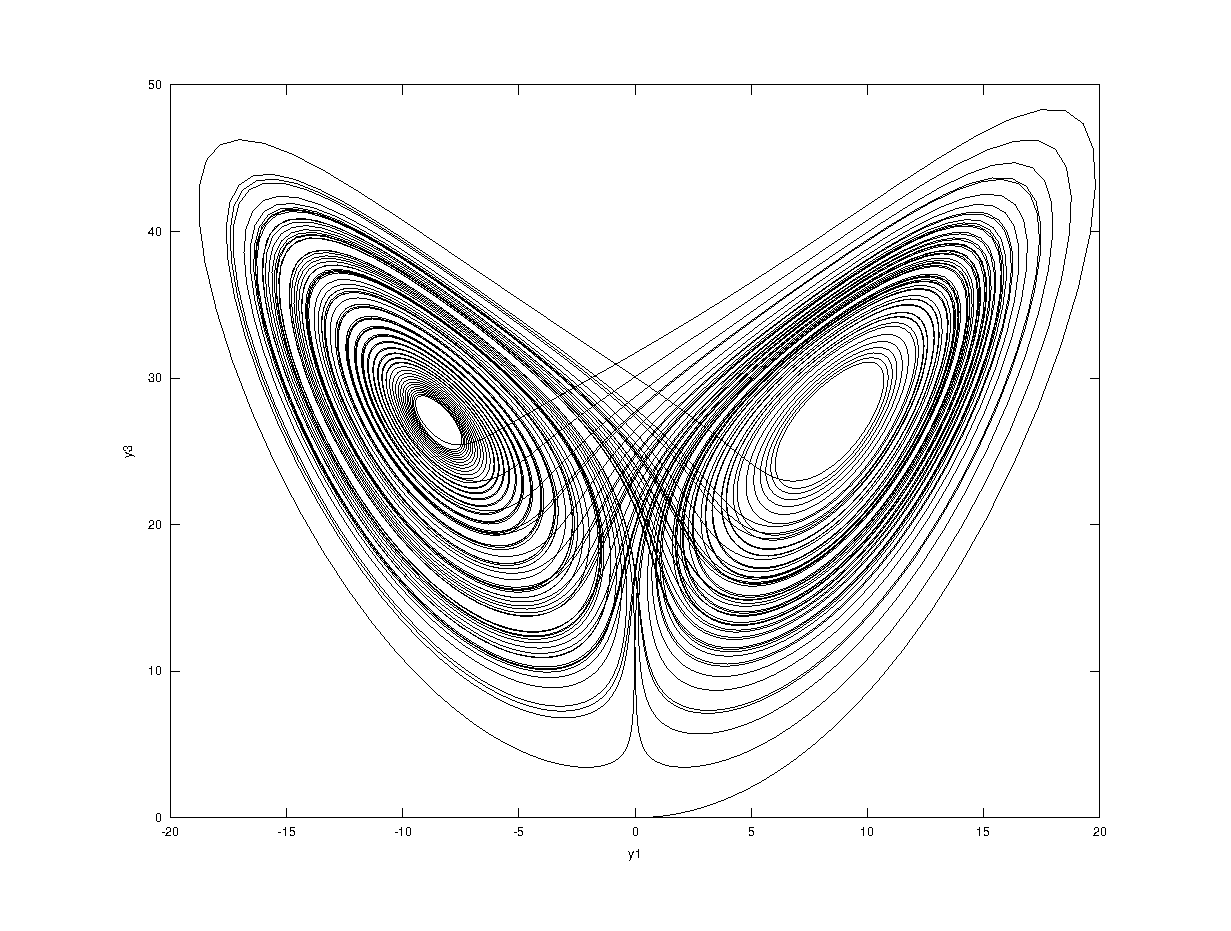
\includegraphics[width=0.65\textwidth]{pp2.eps}
	\end{center}
	\begin{center}
		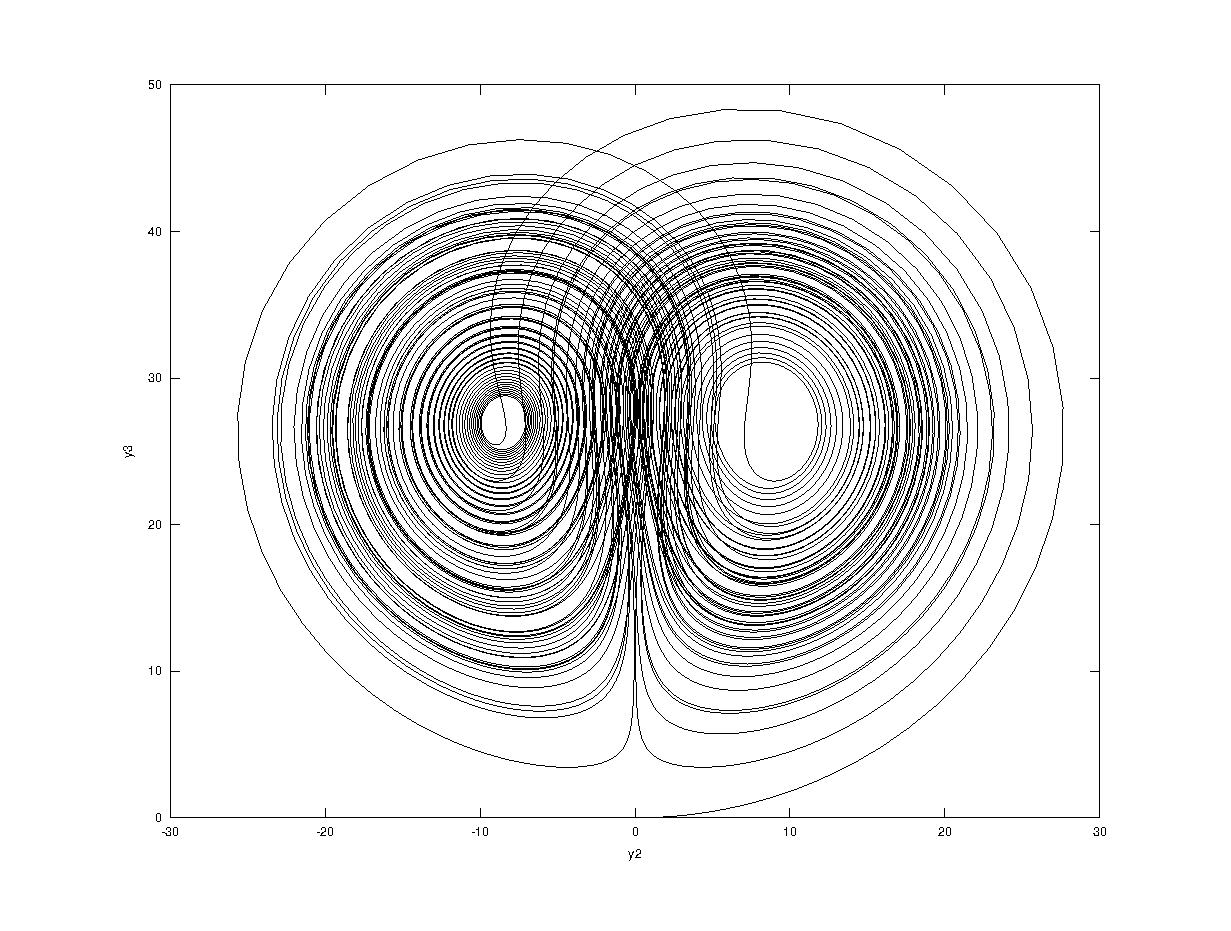
\includegraphics[width=0.65\textwidth]{pp3.eps}
	\end{center}
	
	\item[(c)] 3D plot
		\begin{center}
		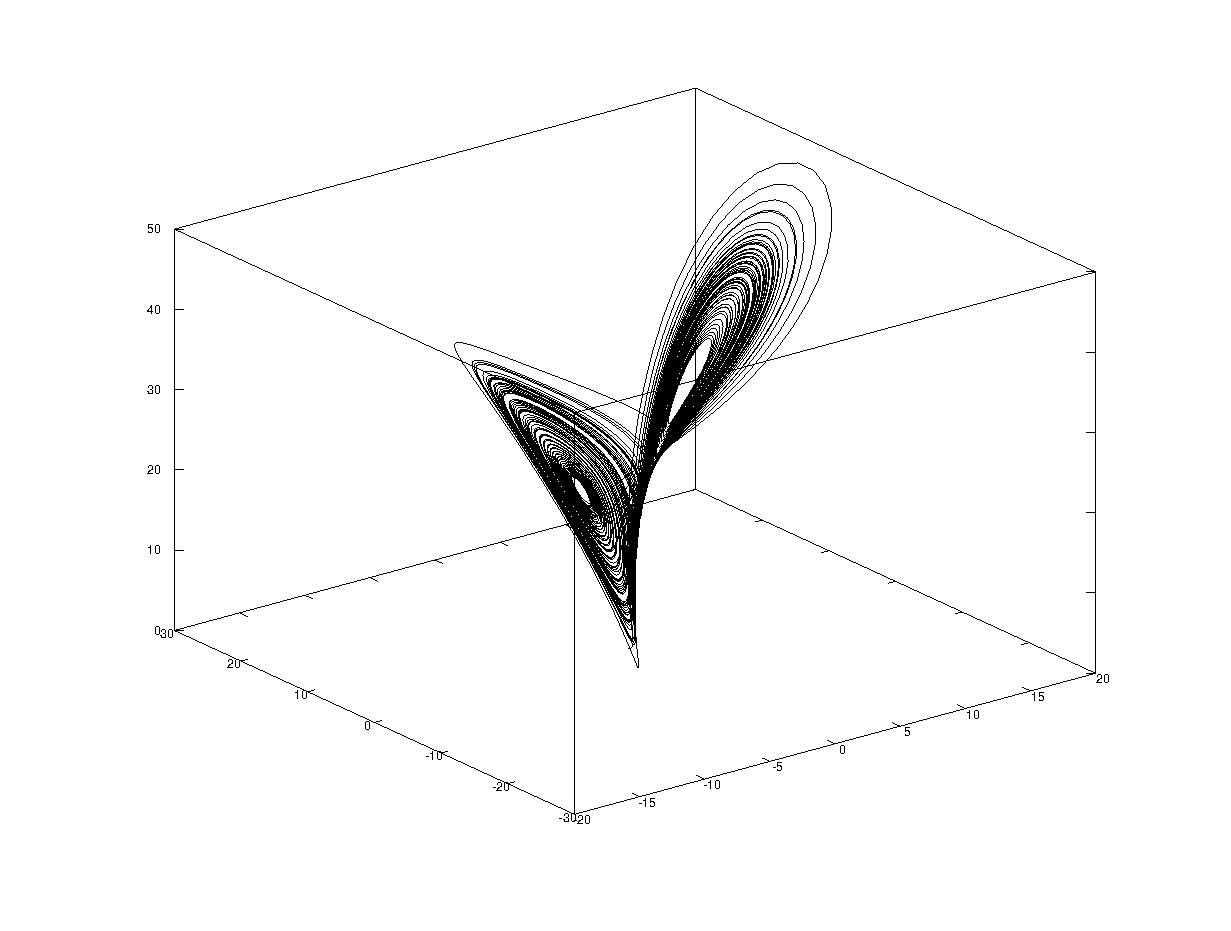
\includegraphics[width=1\textwidth]{threed.eps}
	\end{center}
	
	We then experimented by changing the initial conditions by a tiny amount. Using a random number generator, we changed our initial values from $[y_1(0) \ y_2(0) \ y_3(0)] = [0 \ 1 \ 0]$ to 
	\begin{align*}
		\begin{bmatrix}
			y_1(0) \\ 
			y_2(0) \\
			y_3(0) \\
		\end{bmatrix}=
			\begin{bmatrix}
			-2.7813\text{e}^{-11} \\ 
			1+2.6788\text{e}^{-12} \\
			-3.2696\text{e}^{-11} \\
		\end{bmatrix}
	\end{align*}
	The following table compares the final values under both scenarios.
	\begin{center}
		\begin{tabular}{|c|c|c|}
		\hline
		Final value &Original &Changed \\
		\hline
		$y_1(100)$ &3.7149 &-12.570 \\
		$y_2(100)$ &-2.1299 &-11.581 \\
		$y_3(100)$ &29.570 &33.796 \\ 
		\hline
		\end{tabular}
	\end{center}
	It follows that numerical solutions to differential equations are very sensitive to even the tiniest of changes to initial conditions. We repeat parts (a)-(c) to check for any graphical differences.
	
	\pagebreak
	
	\begin{enumerate}
	\item[(i)] $\textbf{lsode}$ solution under changed initial values
	\begin{center}
		\includegraphics[width=0.65\textwidth]{y1s.eps}
	\end{center}
	\begin{center}
		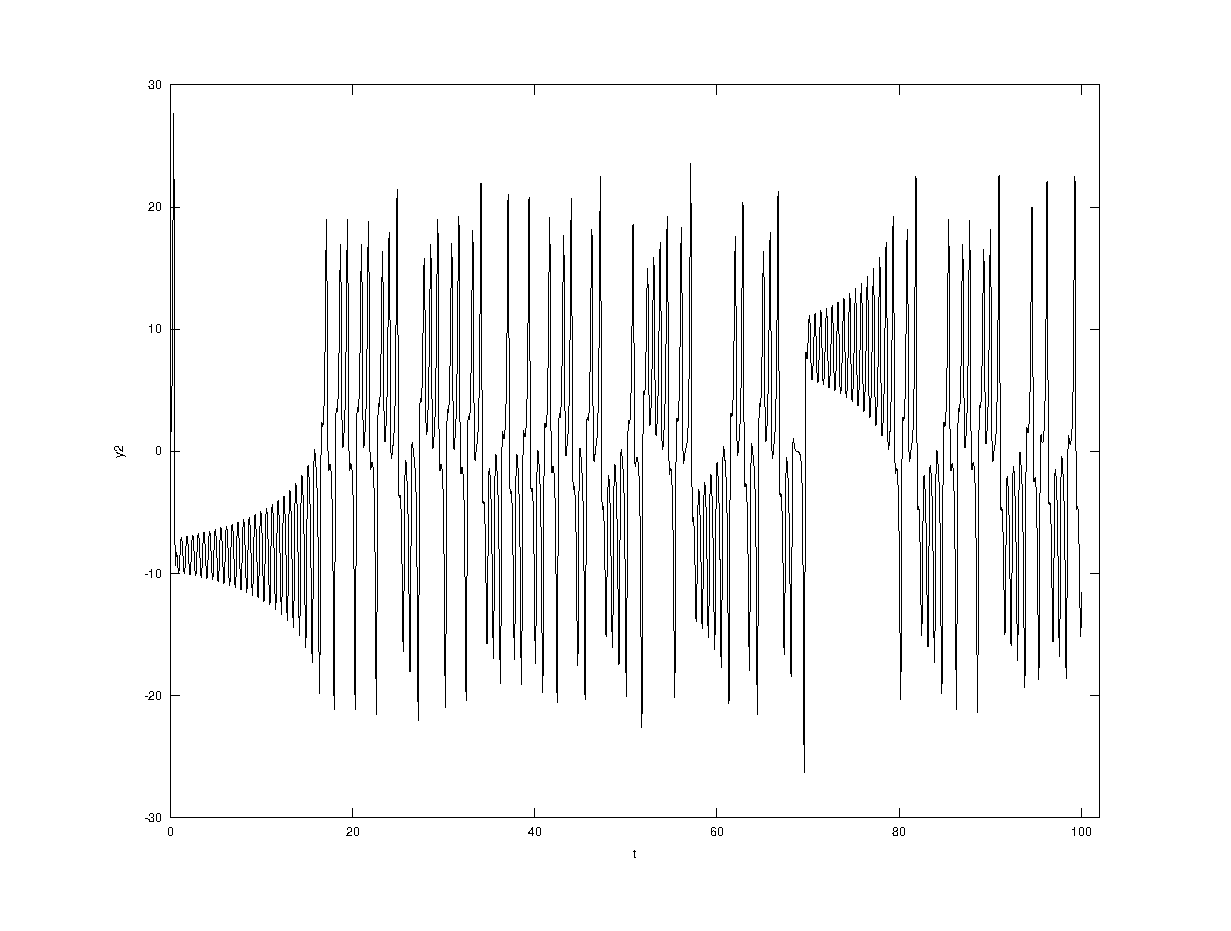
\includegraphics[width=0.65\textwidth]{y2s.eps}
	\end{center}
	\begin{center}
		\includegraphics[width=0.65\textwidth]{y3s.eps}
	\end{center}
	\pagebreak
	
	\item[(ii)] Phase-plane plots under changed initial values
	\begin{center}
		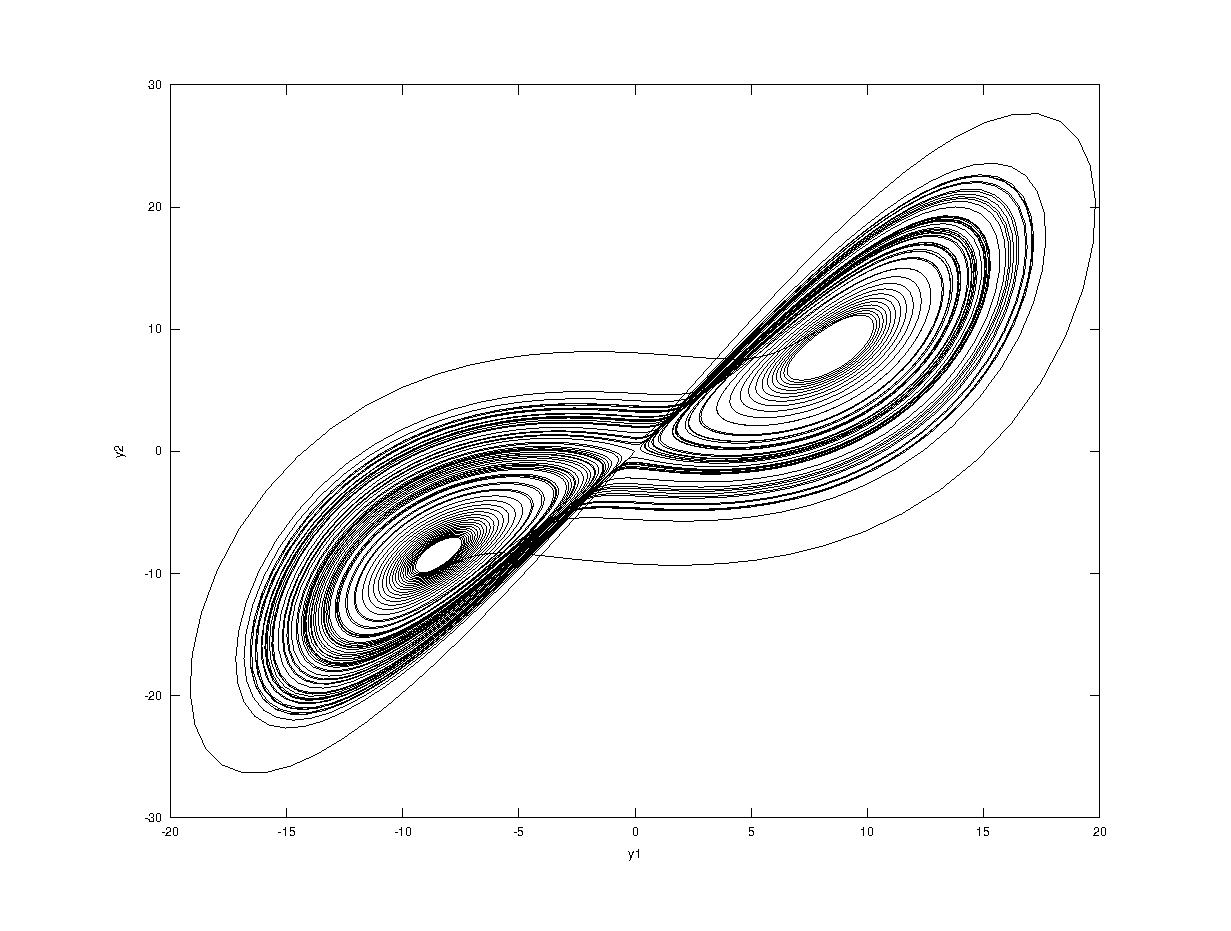
\includegraphics[width=0.65\textwidth]{pp1s.eps}
	\end{center}
	\begin{center}
		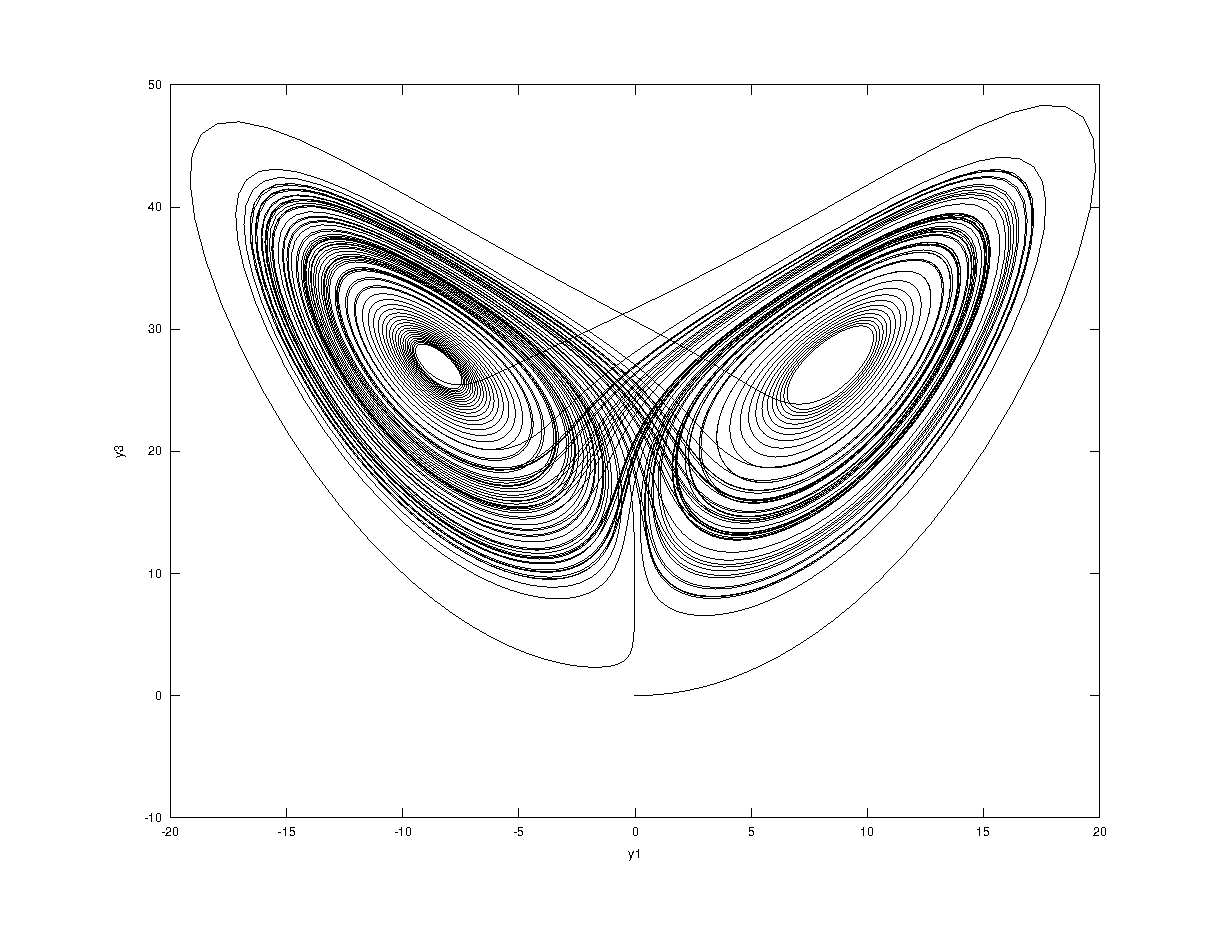
\includegraphics[width=0.65\textwidth]{pp2s.eps}
	\end{center}
	\begin{center}
		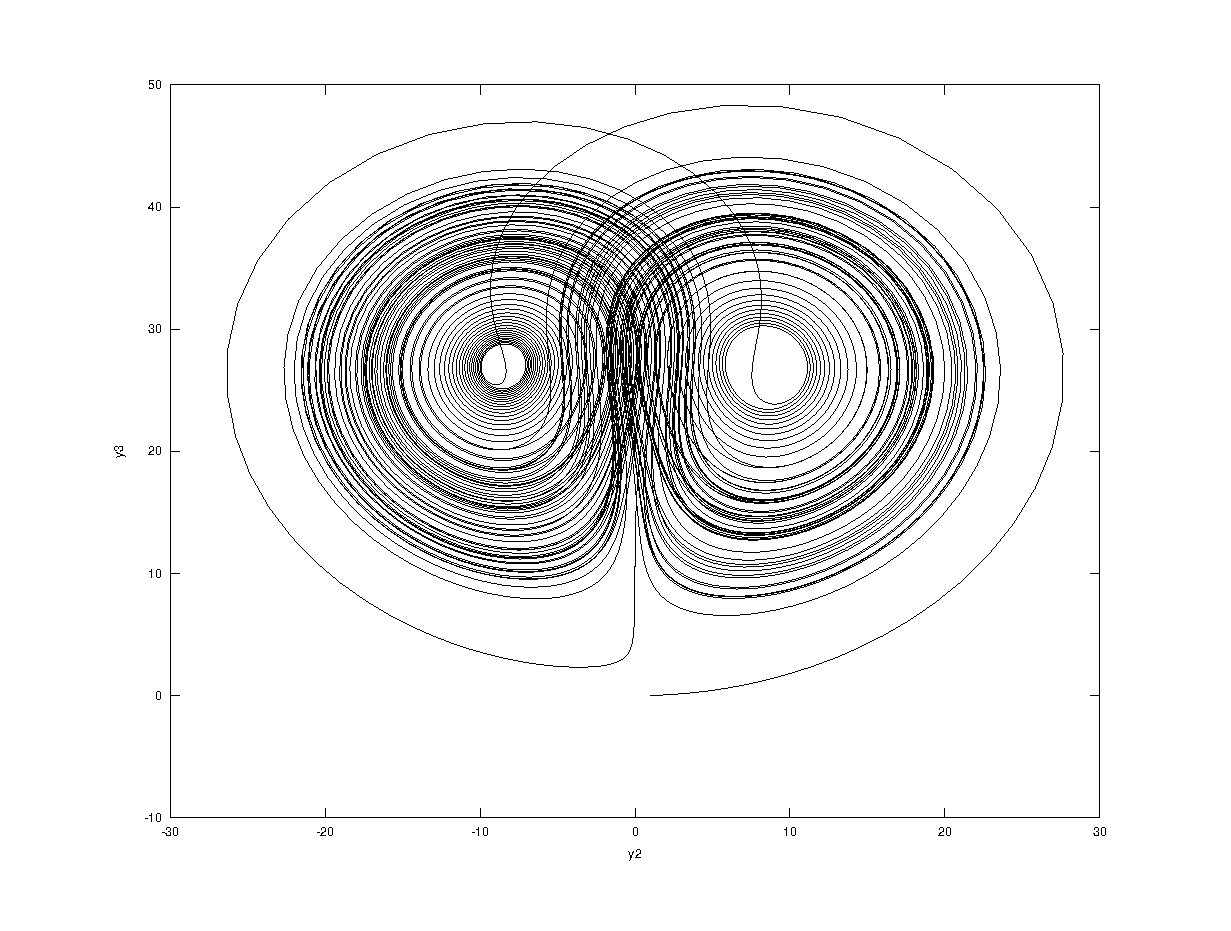
\includegraphics[width=0.65\textwidth]{pp3s.eps}
	\end{center}
	
	\pagebreak
	
	\item[(iii)] 3D plot under changed initial values
		\begin{center}
		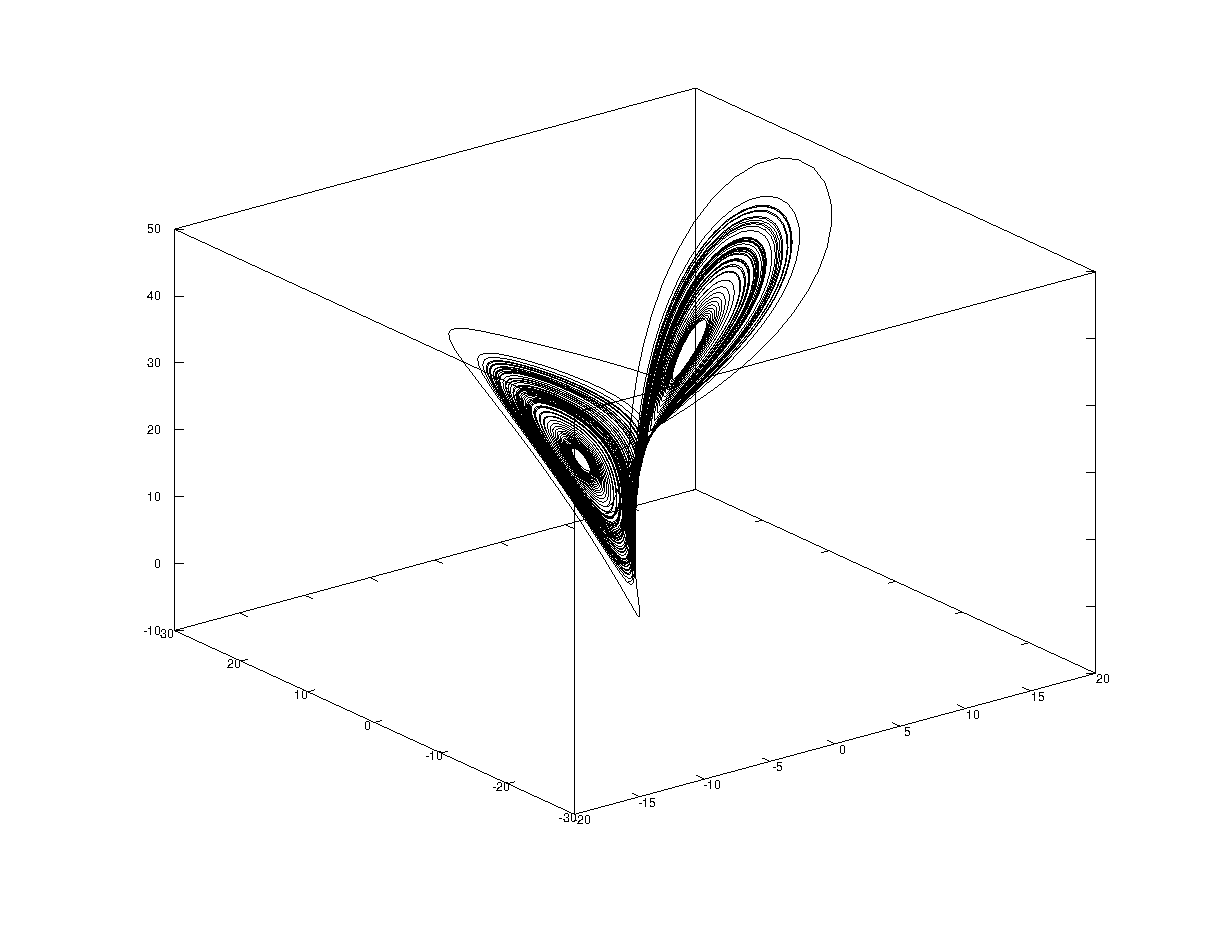
\includegraphics[width=1\textwidth]{threeds.eps}
	\end{center}
	\end{enumerate}
	
	We observe no significant change to the overall shapes and patterns of the phase-plane and 3D plots after changing initial values, except perhaps for minor displacements. However, there are some notable differences in the $\mathbf{y}$ over $t$ plots, particularly for $y_1$ and $y_2$ after $t=50$.
\end{enumerate}

\pagebreak

\textbf{Appendix}

\begin{enumerate}
	\item 
	\begin{enumerate}
		\item
		\begin{verbatim}
			ezplot(f1, [0,15])
			print('f1.eps','-deps')
		\end{verbatim}
		
		\item
		\begin{verbatim}
			ezplot(f2, [-1,1])
			print('f2.eps','-deps')
		\end{verbatim}
		
		\item
		\begin{verbatim}
			ezplot(f3, [0,pi])
			print('f3.eps','-deps')
		\end{verbatim}
	\end{enumerate}
		
	\item
	\begin{verbatim}
		x=-10:0.01:10;
		c=@(x) cos(pi*x.^2/2);
		s=@(x) sin(pi*x.^2/2);
		
		for i=1:length(x)
		C(i)=quad(c,0,x(i));
		S(i)=quad(s,0,x(i));
		end
		
		plot(x,C)
		print('fresc.eps','-deps')
		plot(x,S)
		print('fress.eps','-deps')
		plot(S,C)
		print('cornu.eps','-deps')
	\end{verbatim}
	
	\item
	\begin{enumerate}
		\item
		\begin{verbatim}
			function v = monte4d(n)
			k=0;
			for i=1:n
			x=rand(1,1);
			y=2*rand(1,1);
			z=4*rand(1,1);
			if (x^2+y.^2/4+z.^2/16<=1)
			k=k+1;
			end
			end
			v=64*k/n;
			endfunction
			
			monte4d(100000)
		\end{verbatim}
		
		\pagebreak
		
		\item
		\begin{verbatim}
			function ii=monte2d(n)
			k=0;
			sumf=0;
			while (k<n)
			x=rand(1,1);
			y=rand(1,1);
			if (x.^2+y.^2<=1)
			k=k+1;
			sumf=sumf+exp(-sqrt(x.^2+y.^2));
			end
			end
			ii=(pi/2)*(sumf/n);
			endfunction
			
			monte2d(100000)
		\end{verbatim}
		
	\end{enumerate}
	
	\item 
	\begin{verbatim}
		f=@(t,y) -2*t*y;
		N=16;
		h=zeros(1,N);
		y1=zeros(1,N);
		for k=1:N
		hk=2^-k;
		h(k)=hk;
		[t y]=euler(f,0,1,hk,2^k);
		y1(k)=y(end);
		end
			
		plot(t,y)
		xlabel('t')
		ylabel('y')
		print('euler.eps','-deps')
			
		err=y-exp(-t.^2);
		plot(t,err)
		xlabel('t')
		ylabel('error')
		print('error.eps','-deps')
			
		err1=exp(-1)-y1
		plot(h,err1)
		xlabel('t')
		ylabel('error')
		print('err1.eps','-deps')
	\end{verbatim}
	
	\item
	\begin{verbatim}
		global sigma b r
		sigma=10; 
		b=8/3; 
		r=28;
	
		function dy = lv(y,t)
		global sigma b r
		dy=zeros(3,1);
		dy(1)=sigma*(y(2)-y(1));
		dy(2)=r*y(1)-y(2)-y(1)*y(3);
		dy(3)=y(1)*y(2)-b*y(3);
		endfunction
		
		t=(0:0.01:100)';
		y=lsode(@lv,[0 1 0],t);
	\end{verbatim}
	
	\begin{enumerate}
		\item
		\begin{verbatim}
			plot(t,y(:,1))
			axis([0 102 -20 20])
			xlabel('t')
			ylabel('y1')
			print('y1.eps','-deps')

			plot(t,y(:,2))
			axis([0 102 -30 30])
			xlabel('t')
			ylabel('y2')
			print('y2.eps','-deps')

			plot(t,y(:,3))
			axis([0 102 0 50])
			xlabel('t')
			ylabel('y3')
			print('y3.eps','-deps')
			
		\end{verbatim}
		
		\item
		\begin{verbatim}
			plot(y(:,1),y(:,2))
			xlabel('y1')
			ylabel('y2')
			print('pp1q.eps','-deps')
			
			plot(y(:,1),y(:,3))
			xlabel('y1')
			ylabel('y3')
			print('pp2.eps','-deps')
			
			plot(y(:,2),y(:,3))
			xlabel('y2')
			ylabel('y3')
			print('pp3.eps','-deps')
			
		\end{verbatim}
		
		\item
		\begin{verbatim}
			plot3(y(:,1),y(:,2),y(:,3))
			print('threed.eps','-deps')
			
			c=1e-10*randn(1,1);
			d=1e-10*randn(1,1);
			g=1e-10*randn(1,1);

			t=(0:0.01:100)';
			y1=lsode(@lv,[c 1+d g],t);
			
		\end{verbatim}
		\begin{enumerate}
		\item
		\begin{verbatim}	
			plot(t,y1(:,1))
			axis([0 102 -20 20])
			xlabel('t')
			ylabel('y1')
			print('y1s.eps','-deps')

			plot(t,y1(:,2))
			axis([0 102 -30 30])
			xlabel('t')
			ylabel('y2')
			print('y2s.eps','-deps')

			plot(t,y1(:,3))
			axis([0 102 0 50])
			xlabel('t')
			ylabel('y3')
			print('y3s.eps','-deps')
			
		\end{verbatim}
		
		\item
		\begin{verbatim}
			plot(y1(:,1),y1(:,2))
			xlabel('y1')
			ylabel('y2')
			print('pp1s.eps','-deps')

			plot(y1(:,1),y1(:,3))
			xlabel('y1')
			ylabel('y3')
			print('pp2s.eps','-deps')

			plot(y1(:,2),y1(:,3))
			xlabel('y2')
			ylabel('y3')
			print('pp3s.eps','-deps')
			
		\end{verbatim}
		
		\item
		\begin{verbatim}
			plot3(y1(:,1),y1(:,2),y1(:,3))
			print('threeds.eps','-deps')
		\end{verbatim}
		
		\end{enumerate}
		
	\end{enumerate}
\end{enumerate}

\end{document}